% %%% fs-state-model - Model

\label {fs-model-section}

In this section, we outline the lightweight deterministic model. While it is described in details in~\cite{we2018adbis}, in this paper we mention properties, which play important roles in consistency enforcement techniques.

Set $\Gamma$ of all possible data flow elements in our model consists of {\em data items}. Data item contains an arbitrary application domain {\it payload} and a structured system-assigned {\it meta-information}.

\[DataItem := (Payload, Meta)\]

The exact form of meta-information is detailed in the next section, but its main purposes are:
\begin{itemize}
    \item Define a total order on all data flow elements. The order is used for achieving determinism and deduplication
    \item Maintain information about $Cl^{-1}(D)(x)$ for each data item $x$
    \item Keep extra information about a data item
\end{itemize}

\subsection{Optimistic determinism}

A straightforward approach, how to make stream processing system deterministic, requires several steps:
\begin{enumerate}
    \item Preserve total order defined by meta-information before each order-sensitive operation in a data flow
    \item Preserve the same order of output items
    \item Ensure that all operations are pure
\end{enumerate}

At first glance, total order maintenance is over-restrictive. It can be achieved, e.g., using buffering before each order-sensitive operation until punctuation or low watermark arrives ~\cite{Li:2008:OPN:1453856.1453890}. However, frequent buffering can dramatically increase latency. 

Any logical graph in the drifting state model is constructed using the following two operations:

{\bf Map} applies a user-defined function to the payload of an input item. This function returns a sequence of data items with transformed payloads. An output sequence can be empty.

{\bf Grouping} has a {\it window size} parameter. Grouping stores input items into distinct buckets by the value of the input balancing function applied to the payload. When the next item arrives at the grouping, it is appended to the corresponding bucket. Each time the grouping outputs window-sized {\it tuple item}, which consists of the most recent (in terms of the meta-information) items of this bucket. If the size of the bucket is less than the window, all items of the bucket are taken.

The following example illustrates the semantics of the operation. The grouping accepts items with payload represented as natural numbers: 1,2,3, etc. The hash function returns 1 if the number is even and 0 otherwise. If the window is set to 3, the output elements are:

\[(1), (2), (1|3), (2|4), (1|3|5), (2|4|6), (3|5|7), (4|6|8)...\]

Actually, any stateful transformation can be expressed by decomposing into map and grouping operations with a cycle. Let us illustrate it by the example of sum operation. In a classical setting, each element is combined with previous state value and released. Then, the state is updated. In our model, firstly each element is grouped with previous state element into the pair. After that, map operation delivers a combined result, updates the state, and returns it to the grouping through the cycle. A comparison between the classical state handling approach and the drifting state model is shown in Figure~\ref{classical-drifting}.

\begin{figure}[htbp]
  \centering
  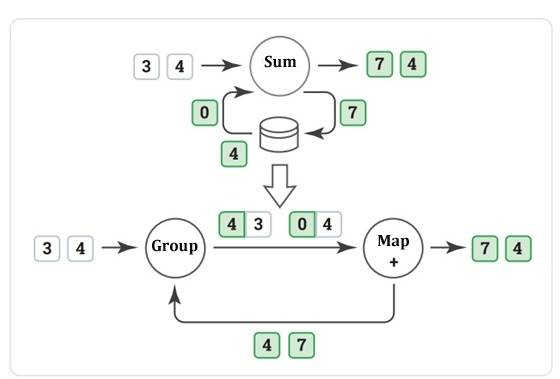
\includegraphics[width=.49\textwidth]{pics/classical-drifting}
  \caption{The comparison between classical state handling approach and drifting state model}
  \label {classical-drifting}
\end{figure}

We call this model a drifting state because operation states become ordinary data flow elements. In this setting, map operation is pure and order insensitive, and grouping operation is pure. Grouping operation is order-sensitive because it should group a new element with the exact previous state. Fortunately, grouping can be implemented optimistically. The scheme is shown in Figure~\ref{optimistic-grouping}. The numbers on this figure represent meta-information. An element with meta 3 is out-of-order. We know that actually invalid pair (one; five) has been already released. In this case, the system generates valid pairs because it knows the right position of the element with meta 3. Besides, an invalid pair with a special flag in meta is resent. Let us call such elements invalidators or tombstones. The purpose of invalidators is to hunt down previously released invalid pairs and to remove them from other grouping or to intercept before delivery to end-user. Map functions are required to be pure in order to ensure that invalidators will go through exactly the same path as original pairs. This method is applicable to any number of subsequent groupings.
 
\begin{figure}[htbp]
  \centering
  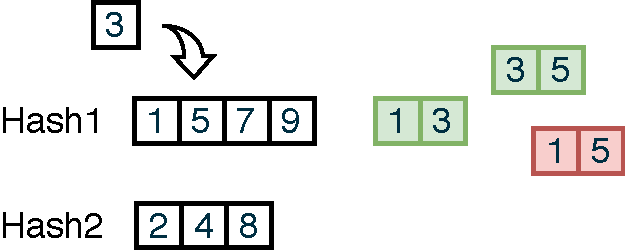
\includegraphics[width=.35\textwidth]{pics/grouping-invalidation}
  \caption{An idea of optimistic grouping implementation}
  \label {optimistic-grouping}
\end{figure} 
 
In order to allow invalidators to catch invalid pairs, we buffer all items before output in a very last node of the graph called a {\em barrier}. The barrier can be safely flushed if there is a guarantee that there are no in-flight invalidators for elements in the barrier. Hence, an element can be released from the barrier at the nullification time of the last input items, which affect it. In other words, element $b$ can be released at the time $\tau(t)$ if $\forall{a}:b\in{Cl(D)(a)},\theta_a \leq \tau(t)$. If there is information, which input elements have been already nullified, meta-information of an element in the barrier can be used to determine the correct moment to release this element. The exact method for barrier flushing is discussed in the next section. Barrier releases items in the order of meta-information, so results will be the same after any number of reruns on the same input. It is worth to note that barrier is the only buffer in any data flow graph within this approach due to optimistic groupings. 

The drifting state has the following properties:
\begin{itemize}
    \item Determinism is achieved by the price of a single buffer per any data flow graph. In our experiments, the waiting time in this buffer is in order of milliseconds~\cite{we2018adbis}.
    \item There are only two operations: map and windowed grouping. The set of dependencies $D$ is generated by these operations.
    \item User-defined code can be present only in map operation, while for grouping, a user should define hash balancing function.
    \item Map is stateless operation and grouping maintains sorted on meta-information lists of data items. The system itself only can manage this state, so the drifting state model is stateless from a user point of view.
    \item In spite of the reduced set of operations, this model is sufficient to express any stateful transformation.
    \item The only requirement of our model is that map operations must be pure.
\end{itemize}

\subsection{Snapshotting}

As it is demonstrated in section~\ref{fs-formalism}, in a deterministic system, state snapshotting and output delivery can be unsynchronized if the system includes in the snapshot last released element as well as system state. The problem here is a need to save at the time $\tau$ snapshot for state $S_{\tau-n}$ for some $n$.

The only stateful operation in the drifting state model is grouping. Hence, there is only a need to save grouping's state in order to take the complete state snapshot. Grouping's state in practice are lists of data items sorted by meta-information. If all input elements $[a_{0}...a_{\tau-n}]$ have been nullified, then state $S_{\tau-n}$ can be snapshotted. Therefore, to take a snapshot at time $\tau$, there is a need to determine maximal $\tau-n$ such that all input elements $[a_{0}...a_{\tau-n}]$ have been nullified. After that, we can just save elements from grouping state lists, which are affected only by these elements. These elements can be determined using meta-information because it contains information about $Cl^{-1}(D)$.

The fact that the only state in the drifting state model has a simple structure of lists sorted by meta-information allows us to take snapshots that contain {\em the past} state. The property of determinism guarantees that such state snapshot together with the last released element is enough to make snapshotting mechanism consistent. The exact protocols, which are used for snapshotting are detailed in the next section.  